\documentclass{beamer}

%%%% Packages
\usepackage{amsmath, amsthm, amssymb}
\usepackage[english]{babel}
\usepackage{array}              % for >{} in table column
% specification
\usepackage{color}              % for color definition
\usepackage{colortbl}
\usepackage{graphicx}
\usepackage{multirow}           % for multirow
\usepackage{multicol}           % for multiple columns
\usepackage{tabularx}           % for centering in table
\usepackage{tikz}               % for drawing diagrams
\usetikzlibrary{arrows}

%%%% Macros and Definitions
\definecolor{firebrick4}{RGB}{139,026,026}
\definecolor{gray57}{RGB}{145,145,145}
\definecolor{gray71}{RGB}{181,181,181}
\definecolor{gray84}{RGB}{212,212,212}
\definecolor{lightcyan4}{RGB}{122,139,139}
\definecolor{dodgerblue4}{RGB}{16,78,139}
\definecolor{dodgerblue3}{RGB}{24,116,205}

\newcommand{\indentpar}[1]{{\setlength{\parindent}{1cm} #1}}

%%%% Presentation Setup
\mode<presentation>
    {
      \usetheme{Ilmenau}
      \usecolortheme{beaver}
      \usefonttheme[onlylarge]{structuresmallcapsserif}
    }
    \setbeamercolor{title}{fg=dodgerblue4}
    \setbeamercolor{frametitle}{fg=dodgerblue4}
    \setbeamercolor*{palette secondary}{fg=dodgerblue4,bg=gray84}
    \setbeamercolor*{palette tertiary}{fg=white,bg=dodgerblue4}
    \setbeamercolor*{item}{fg=dodgerblue4}

    \setbeamerfont{author}{size=\scriptsize}
    \setbeamerfont{institute}{size=\scriptsize}
    \setbeamerfont{date}{size=\tiny}
    \setbeamerfont{normal text}{size=\scriptsize}

    \beamertemplatenavigationsymbolsempty

    %%%% Title
    \title[Bericht 2014]{DASoM Bericht -- September 2014}
    \author[Sidorenko]{Wladimir Sidorenko\\ \texttt{uladzimir.sidarenka{@}uni-potsdam.de}}
    \institute[Uni Potsdam]{University of Potsdam}
    \date{\today}

    \pgfdeclareimage[interpolate=true,height=2.5cm]{logo}{img/uni_potsdam_logo.png}
    \titlegraphic{\pgfuseimage{logo}}

    %%%% Document
    \begin{document}
    %%%%%%%%%%%%%%%%%%%%%%%%%%%%%%%%%%%%%%%%%%%%%%%%%%%%%%%%%%%%%%%%%%
    %%% Title Page
    \begin{frame}{}
      \titlepage
    \end{frame}

    %%%%%%%%%%%%%%%%%%%%%%%%%%%%%%%%%%%%%%%%%%%%%%%%%%%%%%%%%%%%%%%%%%
    %%% Table of Contents
    \begin{frame}{Inhaltsverzeichnis}
      \tableofcontents
    \end{frame}

    %%%%%%%%%%%%%%%%%%%%%%%%%%%%%%%%%%%%%%%%%%%%%%%%%%%%%%%%%%%%%%%%%%
    %%% Sentiment Corpus
    \section{Sentiment Korpus}
    \subsection{Auswahlkriterien}
    \begin{frame}{\insertsubsection}
      Zum Entwickeln und Testen unseres Sentimentsystems, wurde ein Korpus von
      4995 Twitter-Nachrichten erstellt.  Dieses Korpus setzt sich zusammen
      aus Tweets zu vier gro\ss{}en Themen (zwei politische und zwei nicht
      politische), wobei f\"ur jedes Thema die Nachrichten nach jeweils drei
      unterschiedlichen formellen Kriterien ausgew\"ahlt wurden.
    \end{frame}

    \begin{frame}{\insertsubsection}
      Die ausgew\"ahlten Themen waren:
      \begin{enumerate}
      \item Politische:
        \begin{itemize}
        \item Tweets \"uber politische Akteure {\tiny(M\"arz 27 -- Mai 25,
          2013)};
        \item Tweets \"uber die Bundestagswahl 2013 {\tiny(Juni 15 --
          September 30, 2013)};
        \end{itemize}

      \item Nicht politische:
        \begin{itemize}
        \item Allgemeine Tweets zu keinem bestimmten Thema {\tiny(M\"arz
          31 -- April 30, 2013)};
        \item Tweets zum Thema Papstwahl 2013 {\tiny(M\"arz 13 -- M\"arz 14,
          2013)}.
        \end{itemize}
      \end{enumerate}
    \end{frame}

    \begin{frame}{\insertsubsection}
      Formelle Kriterien waren:
      \begin{enumerate}
      \item Vorhandensein eines polaren Terms (SentiWS \cite{Remus-10});
      \item Pr\"asenz von Emoticons und Ausrufezeichen;
      \item Zuf\"allige Auswahl in restlichen Nachrichten.
      \end{enumerate}
      F\"ur jedes der obengenannten Kriterien wurden 333 Tweets f\"ur jedes
      Thema ausgew\"ahlt.
    \end{frame}

    \subsection{Annotationsschema}
    \begin{frame}{\insertsubsection}
      \textbf{Emo-expressions} (\textit{expressive subjective elements}
      \cite{Wiebe-05}) - W\"orter und Wendungen mit polarem subjektiver
      Einsch\"atzung, z.B. \textit{gut, schrecklich, kritisieren, zum Besten
        halten usw.};

      \textbf{Diminishers} (\textit{down-turners} \cite{Taboada-11}) -
      W\"orter und Wendungen, die die Intensit\"at von
      \textit{emo-expressions} herabsetzen, z.B. \textit{weniger, bisschen,
        kaum usw.}

      \textbf{Intensifiers} - W\"orter, die den polaren einsch\"atzenden Sinn
      von \textit{emo-expressions} verst\"arken, z.B. \textit{recht, super,
        au\ss{}erordentlich usw.}

      \textbf{Negations} - Sprachelemente, die die Polarit\"at von
      einsch\"atzenden subjektiven Ausdr\"ucken ins Gegenteil umkehren,
      z.B. \textit{nicht, kein, usw.}
    \end{frame}

    \begin{frame}{\insertsubsection}
      \textbf{Sentiment} - minimale vollst\"andige zusammenh\"angen
      syntactische oder Diskurselemente, die die Bewertung einer Person,
      Organisation oder eines bestimmten Themas oder Ereignisses ausdr\"ucken,
      z.B. \textit{Ich hasse diese Reform}, \textit{ein ausgezeichneter Film},
      \textit{Meine Mutter ruft mich heulend an.  Denn man hat einen
        Argentinier zum Papst gew\"ahlt.};

      \textbf{Source} - der unmittelbare Autor einer polaren einsch\"atzenden Meinung;

      \textbf{Target} - Objekt oder Ereignis, das von der bewertenden Meinung
      charakterisiert wird.
    \end{frame}

    \begin{frame}{\insertsubsection}
      \begin{example}
        \begin{math}
        [[\text{Ich}]_{\text{\bfseries source}}
          [\text{hasse}]_{\text{\bfseries emo-expression}}
          [\text{Merkel}]_{\text{\bfseries target}}]_{\text{\bfseries sentiment}}\text{.}
        \end{math}
      \end{example}
    \end{frame}

    \subsection{$\kappa$-Agreement}
    \begin{frame}{\insertsubsection}
      \begin{table}
        \caption{\scriptsize $\kappa$ Agreement f\"ur Sentiment-Korpus I.}
        \centering
        \begin{tabular}{p{0.18\textwidth}*{5}{>{\centering\arraybackslash}p{0.13\textwidth}}}
          \hline\noalign{\smallskip}
          \multirow{2}{*}{Element} & %
          \multicolumn{2}{c}{\texttt{Politics}} & %
          \multicolumn{2}{c}{\texttt{Non-politics}} & Gesamt\\
          & Politik & Wahlen & Allgemein & Papstwahl\\
          \noalign{\smallskip} \hline
          Sentiment & 0.35 & 0.35 & 0.38 & 0.45 & 0.39\\
          Source & 0.39 & 0.27 & 0.28 & 0.41 & 0.37\\
          Target & 0.32 & 0.38 & 0.28 & 0.4 & 0.38\\
          Emo-expression & 0.64 & 0.57 & 0.72 & 0.68 & 0.64\\
          Diminisher & 0.67 & 0.44 & 0.8 & 0.0 & 0.37\\
          Intensifier & 0.46 & 0.48 & 0.73 & 0.21 & 0.52\\
          Negation & 0.44 & 0.1 & 0.21 & 0.36 & 0.28\\
          \noalign{\smallskip} \hline
        \end{tabular}
      \end{table}
    \end{frame}

    \subsection{$\kappa$-Agreement}
    \begin{frame}{\insertsubsection}
      \begin{table}
        \caption{\scriptsize $\kappa$ Agreement f\"ur Sentiment-Korpus II.}
        \centering
        \begin{tabular}{p{0.15\textwidth}*{5}{>{\centering\arraybackslash}p{0.13\textwidth}}}
          \hline\noalign{\smallskip}
          \multirow{2}{*}{Element} & %
          \multicolumn{2}{c}{\texttt{Politics}} & %
          \multicolumn{2}{c}{\texttt{Non-politics}} & Gesamt\\
          & Politik & Wahlen & Allgemein & Papstwahl\\
          \noalign{\smallskip} \hline
          Sentiment & 0.66 & 0.72 & 0.73 & 0.68 & 0.7\\
          Source & 0.72 & 0.77 & 0.71 & 0.69 & 0.73\\
          Target & 0.61 & 0.71 & 0.7 & 0.65 & 0.68\\
          Emo-expression & 0.83 & 0.84 & 0.88 & 0.86 & 0.86\\
          Diminisher & 0.67 & 0.64 & 0.62 & 0.18 & 0.53\\
          Intensifier & 0.51 & 0.62 & 0.6 & 0.37 & 0.56\\
          Negation & 0.55 & 0.58 & 0.6 & 0.66 & 0.6\\
          \noalign{\smallskip} \hline
        \end{tabular}
      \end{table}
    \end{frame}

    %%%%%%%%%%%%%%%%%%%%%%%%%%%%%%%%%%%%%%%%%%%%%%%%%%%%%%%%%%%%%%%%%%
    %%% Sentiment Analysis
    \section{Sentiment Analyse}
    \subsection{Klassifikatoren}
    \begin{frame}{\insertsubsection}
      \begin{table}
        \caption{\scriptsize Klassifikationsergebnisse f\"ur automatische
          Sentimentanalyse (Token-basiert).}
        \centering
        \begin{tabular}{p{0.25\textwidth}*{4}{>{\centering\arraybackslash}p{0.15\textwidth}}}
          \hline\noalign{\smallskip}
          ML-System& Sentiment & Source & Target & Other\\\hline
          SVM & 3.4 & 10.7 & 0 & 94.5\\
          Bayes Net & 15.7 & 9.4 & 5.8 & 89\\
          NB & 15.9 & 7.5 & 8.9 & 78.4\\
          Multinomial NB & 17.5 & 9.8 & 11 & 85.6\\
          CRF & 16.53 & 17.65 & 7.89 & 94.47\\
          \noalign{\smallskip} \hline
        \end{tabular}
      \end{table}
    \end{frame}

    \subsection{CRF}
    \begin{frame}{\insertsubsection}
      Features:
      \begin{multicols}{2}
        \begin{itemize}
        \item Formelle:
          \begin{itemize}
            \tiny
          \item Erste drei Buchstaben der Wortform;
          \item Letzte drei Buchstaben der Wortform;
          \item Buchstabenklasse des Wortes (title, upper, lower, alphabetic
            mixed, alnum, digit, punct, mixed);
          \end{itemize}
        \item Morphologische:
          \begin{itemize}
            \tiny
          \item Kasus;
          \item Genus;
          \item Vergleichsstufe;
          \item Modus;
          \item Tempus;
          \item Person;
          \end{itemize}
        \item Lexikalische:
          \begin{itemize}
            \tiny
          \item Wortform;
          \item Polarit\"atswert (SentiWS* \cite{Remus-10} and
            GermanPolarityClues \cite{Waltinger-10});
          \item Klasse des Modalverbs (lexikalisch oder modal);
          \end{itemize}
        \item Syntaktische:
          \begin{itemize}
            \tiny
            \item Dependenzrelation des vorhergehenden und aktuellen Wortes;
            \item Dependenzrelation des aktuellen Wortes;
            \item Dependenzrelation des aktuellen und n\"achsten Wortes;
            \item Lemma des Mutterknotens;
            \item PoS-Tag der Gro\ss{}mutter;
            \item Form der Gro\ss{}mutter;
            \item Polarit\"atsklasse der Gro\ss{}mutter;
            \item Kind-Lemma + Dependenzrelation;
            \item Kind-Lemma + Dependenzrelation + Lemma;
            \item Kind PoS-Tag + Dependenzrelation + PoS-Tag;
            \item Gesamtpolarit\"atsklasse der Kinder (Polarit\"atsklasse der
              Summe von Polarit\"atswerten der Kinder);
          \end{itemize}
        \end{itemize}
      \end{multicols}
    \end{frame}

    \subsection{Evaluation}
    \begin{frame}{\insertsubsection}
      Evaluationsschemata:
      \begin{itemize}
        \scriptsize
        \item Bin\"are \"Uberlappung \cite{Breck-07}:\\
          \begin{math}\textstyle
            \text{Precision} = \frac{|\left\{p| p \in P \wedge \exists
              c \in C \text{ s.t. } f(c,p)\right\}|}{|P|}\text{; }
            \text{Recall} = \frac{|\left\{c| c \in C \wedge \exists p
              \in P \text{ s.t. } f(c,p)\right\}|}{|C|};
          \end{math}\\
          wo $C$ die Menge der richtigen Spannen ist, $P$ die Menge der
          erkannten Spannen bedeutet, und $f(c, p)$ eine Funktion ist, die
          ``true'' liefert, wenn die Spannen sich \"uberlapen, und sonst
          ``false'' ausgibt;
        \item Proportionale \"Uberlappung \cite{Johansson-10}:\\
          \begin{math}\textstyle
            \text{Precision} = \frac{\text{Score}(C, P)}{|P|}\text{;
            }\text{Recall} = \frac{\text{Score}(P, C)}{|C|};
          \end{math}\\
          wo $\text{Score}(S, S') = \sum_{s \in S}\sum_{s' \in
            S'}f(s, s')$ und $f(s, s') = \frac{|s \cap s'|}{|s'|}$;
        \item Exaktes Matchen \cite{Breck-07}:\\ das Gleiche wie bin\"are
          \"Uberlappung au\ss{}er dass $f(c, p)$ nur dann ``true'' liefert,
          wenn verglichene Spannen in ihren Grenzen v\"ollig einig sind.
      \end{itemize}
    \end{frame}

    \begin{frame}{\insertsubsection}
      \begin{table}
        \tiny
        \caption{\scriptsize Klassifikationsergebnisse f\"ur automatische
          Sentimentanalyse (bin\"are \"Uberlappung, Korpus I). \visible<2>{\alert{Sentiment ist ESE}}}  \centering
        \begin{tabular}{p{0.25\textwidth}*{3}{>{\centering\arraybackslash}p{0.15\textwidth}}}
          \hline\noalign{\smallskip}
          Element & Precision & Recall & F-Ma\ss\\\hline
          \multicolumn{4}{c}{\cellcolor{lightcyan4}Training Set}\\
          \alt<1>{
            Sentiment & 99.23 & 86.27 & 92.29\\
            Source & 91.56 & 75.55 & 82.78\\
            Target & 95.99 & 75.69 & 84.64\\
          }{
            Sentiment & 94.38 & 81.43 & 87.43\\
            Source & 92.31 & 48.54 & 63.62\\
            Target & 96.95 & 56.83 & 71.66\\
          }
          \hline\multicolumn{4}{c}{\cellcolor{lightcyan4}Test Set}\\
          \alt<1>{
            Sentiment & 25 & 16.04 & 19.55\\
            Source & 47.06 & 25 & 32.65\\
            Target & 31.51 & 18.11 & 23\\
          }{
            Sentiment & 76.54 & 68.5 & 72.29\\
            Source & 25 & 18.75 & 21.43\\
            Target & 15.46 & 11.81 & 13.39\\
          }
          \noalign{\smallskip} \hline
        \end{tabular}
      \end{table}
    \end{frame}

    \begin{frame}{\insertsubsection}
      \begin{table}
        \tiny
        \caption{\scriptsize Klassifikationsergebnisse f\"ur automatische
          Sentimentanalyse (proportionale \"Uberlappung, Korpus I). \visible<2>{\alert{Sentiment ist ESE}}}\centering
        \begin{tabular}{p{0.25\textwidth}*{3}{>{\centering\arraybackslash}p{0.15\textwidth}}}
          \hline\noalign{\smallskip}
          Element & Precision & Recall & F-Ma\ss\\\hline
          \multicolumn{4}{c}{\cellcolor{lightcyan4}Training Set}\\
          \alt<1>{
            Sentiment & 97.62 & 84.94 & 90.84\\
            Source & 90.4 & 73.71 & 81.21\\
            Target & 93.55 & 74.02 & 82.65\\
          }{
            Sentiment & 93.62 & 80.5 & 86.57\\
            Source & 92.07 & 48.26 & 63.33\\
            Target & 94.39 & 55.58 & 69.96\\
          }
          \hline\multicolumn{4}{c}{\cellcolor{lightcyan4}Test Set}\\
          \alt<1>{
            Sentiment & 21.31 & 14.53 & 17.28\\
            Source & 40 & 25 & 30.77\\
            Target & 26.06 & 13.75 & 18\\
          }{
            Sentiment & 74.38 & 67.27 & 70.65\\
            Source & 22.22 & 18.75 & 20.34\\
            Target & 12.16 & 10.56 & 11.3\\
          }
          \noalign{\smallskip} \hline
        \end{tabular}
      \end{table}
    \end{frame}

    \begin{frame}{\insertsubsection}
      \begin{table}
        \tiny
        \caption{\scriptsize Klassifikationsergebnisse f\"ur automatische
          Sentimentanalyse (bin\"are \"Uberlappung, Korpus II). \visible<2>{\alert{Sentiment ist ESE}}}  \centering
        \begin{tabular}{p{0.25\textwidth}*{3}{>{\centering\arraybackslash}p{0.15\textwidth}}}
          \hline\noalign{\smallskip}
          Element & Precision & Recall & F-Ma\ss\\\hline
          \multicolumn{4}{c}{\cellcolor{lightcyan4}Training Set}\\
          \alt<1>{
            Sentiment & 99.23 & 86.27 & 92.29\\
            Source & 91.56 & 75.55 & 82.78\\
            Target & 95.99 & 75.69 & 84.64\\
          }{
            Sentiment & 94.38 & 81.43 & 87.43\\
            Source & 92.31 & 48.54 & 63.62\\
            Target & 96.95 & 56.83 & 71.66\\
          }
          \hline\multicolumn{4}{c}{\cellcolor{lightcyan4}Test Set}\\
          \alt<1>{
            Sentiment & 25 & 16.04 & 19.55\\
            Source & 47.06 & 25 & 32.65\\
            Target & 31.51 & 18.11 & 23\\
          }{
            Sentiment & 76.54 & 68.5 & 72.29\\
            Source & 25 & 18.75 & 21.43\\
            Target & 15.46 & 11.81 & 13.39\\
          }
          \noalign{\smallskip} \hline
        \end{tabular}
      \end{table}
    \end{frame}

    \begin{frame}{\insertsubsection}
      \begin{table}
        \tiny
        \caption{\scriptsize Klassifikationsergebnisse f\"ur automatische
          Sentimentanalyse (proportionale \"Uberlappung, Korpus II). \visible<2>{\alert{Sentiment ist ESE}}}\centering
        \begin{tabular}{p{0.25\textwidth}*{3}{>{\centering\arraybackslash}p{0.15\textwidth}}}
          \hline\noalign{\smallskip}
          Element & Precision & Recall & F-Ma\ss\\\hline
          \multicolumn{4}{c}{\cellcolor{lightcyan4}Training Set}\\
          \alt<1>{
            Sentiment & 97.62 & 84.94 & 90.84\\
            Source & 90.4 & 73.71 & 81.21\\
            Target & 93.55 & 74.02 & 82.65\\
          }{
            Sentiment & 93.62 & 80.5 & 86.57\\
            Source & 92.07 & 48.26 & 63.33\\
            Target & 94.39 & 55.58 & 69.96\\
          }
          \hline\multicolumn{4}{c}{\cellcolor{lightcyan4}Test Set}\\
          \alt<1>{
            Sentiment & 21.31 & 14.53 & 17.28\\
            Source & 40 & 25 & 30.77\\
            Target & 26.06 & 13.75 & 18\\
          }{
            Sentiment & 74.38 & 67.27 & 70.65\\
            Source & 22.22 & 18.75 & 20.34\\
            Target & 12.16 & 10.56 & 11.3\\
          }
          \noalign{\smallskip} \hline
        \end{tabular}
      \end{table}
    \end{frame}

    \begin{frame}{Lernkurve}
      \begin{figure}
        \centering
        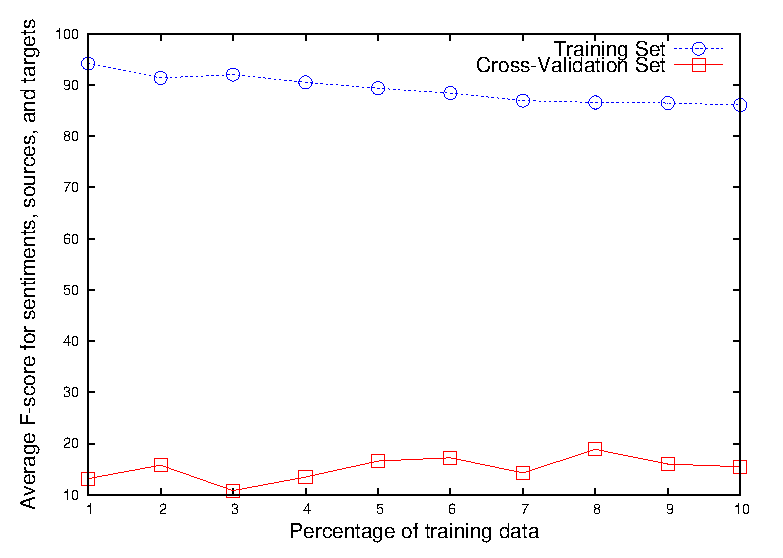
\includegraphics[width = 0.9\textwidth,height=170px]{img/lrn_curve.eps}
      \end{figure}
    \end{frame}

    \section{Diskursanalyse des Twitter-Netzwerks}
    \subsection{Korpus}
    \begin{frame}{\insertsubsection}
      \"Offentliche Diskurse zu allgemeinen und politischen Themen.
    \end{frame}

    \subsection{Annotationsschema und -Tools}
    \begin{frame}{\insertsubsection}
      Relationen:
      \begin{itemize}
        \item Inter-tweet Relationen;
        \item Intra-tweet Relationen;
      \end{itemize}

      Tool:\\ Anpassung des RST-Tools von Daniel Marcu an das Format der
      \"offentlichen Diskurse.
    \end{frame}

    \section*{Bibliography}
    \bibliography{bibliography}
    \bibliographystyle{plain}
    \end{document}
